\chapter{Глубокое обучение}

Лектор: Алексей Сергеевич Забашта

\begin{remark}
    Современное глубокое обучение основано на автоматическом дифференцировании, о котором речь шла на прошлой лекции.
\end{remark}

\section{Послойные архитектуры}

Заметим, что геометрический смысл знака скалярного произведения заключается в том, что он показывает, с какой стороны от гиперплоскости расположена точка.

\begin{remark}
    Даже простые логические функции могут не быть линейно разделимы (не путать с \textit{линейностью} из дискретной математики). Пример логической функции, которая не является линейно разделимой --- $\mathrm{XOR})$.
\end{remark}

Для аппроксимации функций можно использовать сети из линейных преобразований:
\begin{table}[htb]
    \centering
    \begin{tabular}{|r|c|}
        \hline
        AND & $x^1\land x^2=[x^1+x^2-\frac{3}{2}>0]$ \\ \hline
        OR  & $x^1\lor x^2=[x^1+x^2-\frac{1}{2}>0]$  \\ \hline
        NOT & $\neg x=[-x+\frac{1}{2}>0]$            \\ \hline
    \end{tabular}
\end{table}

XOR представляется как композиция, поэтому его также можно записать в таком виде:
\[
    x^1\vee x^2=[(x^1\lor x^2)-(x^1\land x^2)-\dfrac{1}{2}>0]=[x^1+x^2-2x^1x^2-\dfrac{1}{2}>0]
\]

\begin{figure}[htb]
    \centering
    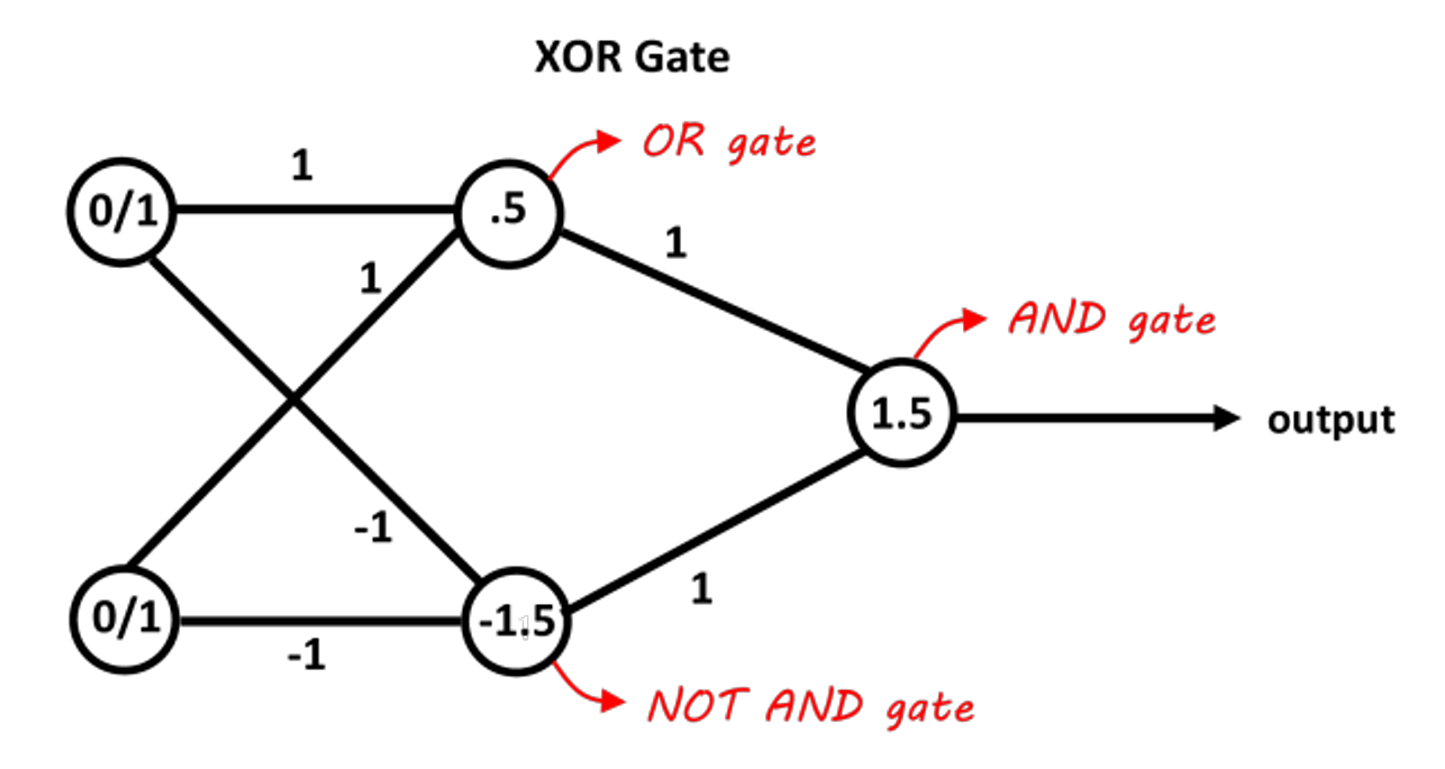
\includegraphics[scale=0.3]{./images/xor-graph.png}
    \caption{Пример для XOR}
\end{figure}

Идея построения композиций из таких преобразований приводит к идее построения многослойных сетей. Каждый слой в них выполняет три операции:
\begin{enumerate}
    \item Умножение на матрицу $A$
    \item Сдвиг вектором $b$
    \item Применение функции активации $\sigma$
\end{enumerate}

\begin{remark}
    Функция активации требуется, чтобы все слои нельзя было свести к одному линейному преобразованию.
\end{remark}

\begin{figure}[htb]
    \centering
    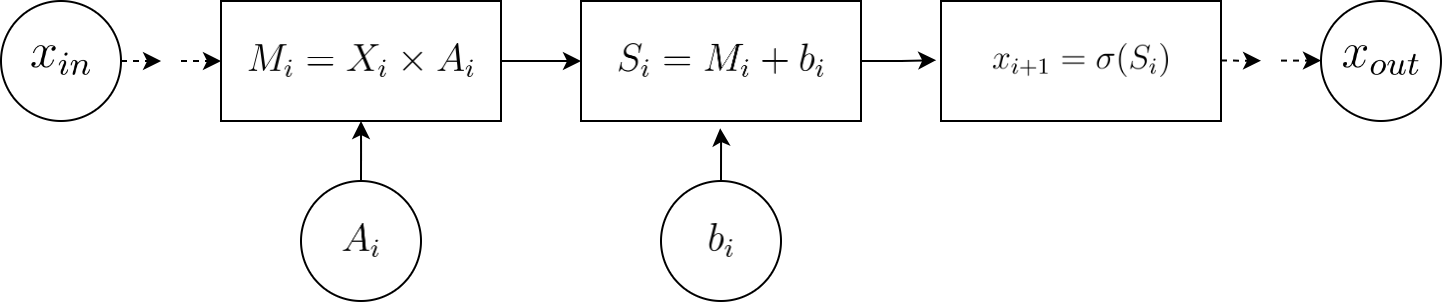
\includegraphics[scale=0.27]{images/matrix-net.png}
    \caption{Матричный вид}
\end{figure}

Одно из преимуществ такого подхода состоит в том, то очень легко контролировать число параметров модели и контролировать недообучение/переобучение. Помимо этого в таком виде очень легко считать производную, используя метод автоматического дифференцирования. Более того, данный процесс можно выполнить параллельно на видеокарте.\newline
Такая архитектура имеет много названий:
\begin{itemize}
    \item \textbf{Mutlilayer Neural Network} (\textit{многослойная нейронная сеть})
    \item \textbf{Fully connected neural network} (\textit{FCNN}, \textit{полносвязная нейронная сеть})
    \item \textbf{Feedforward neural network} (\textit{FNN}, \textit{нейронная сеть с прямой связью})
    \item \textbf{MultiLayer Perceptron} (\textit{MLP}, \textit{многослойный перцептрон})
    \item \textbf{Deep Neural Network} (\textit{DNN}, \textit{глубокая нейронная сеть})
    \item \textbf{Artificial Neural Network} (\textit{ANN}, \textit{искусственная нейронная сеть})
\end{itemize}

Преимущества такой архитектуры заключаются в следующем:
\begin{enumerate}
    \item Для \textbf{логических} функций: любую логическую функцию можно представить в виде ДНФ и КНФ. Следовательно, требуется не более двух слоёв, но с возможно экспоненциальным числом вершин на промежуточном слое.
    \item Для \textbf{числовых} функций: Теорема Цыбенко или Универсальная теорема аппроксимации (1989). Искусственная нейронная сеть с одним скрытым слоем может аппроксимировать любую непрерывную функцию многих переменных с любой точностью при условии достаточного числа вершин на скрытом слое.
\end{enumerate}

\begin{remark}
    В любом случае процесс больше похож на интерполяцию, чем на аппроксимацию. На практике используют больше двух слоев.
\end{remark}

Недостатки:
\begin{enumerate}
    \item При перестановки вершин вместе с весами их ребер функция не меняется (проблема симметрии).
    \item Перестановка может быть непрерывной, следовательно уже для двух слоев функция содержит много минимумов, функция ошибки не будет выпуклой.
    \item \textbf{Проблема затухания градиента} (\textit{vanishing gradient problem}): с каждым слоем градиент затухает. Чем дальше блок от выхода, тем хуже он обучается.
    \item \textbf{Проблема "взрыва" (разрастания) градиента} (\textit{exploding gradient problem}): с каждым слоем градиент может неограниченно расти. Иногда возникает, если присутствует выброс. При обновлении вектор параметров может быть испорчен.
\end{enumerate}

\begin{remark}
    Чтобы уменьшить влияние того факта, что у функции с такой архитектурой много минимумов, можно инициализировать параметры случайными значениями. Например, из нормального или равномерного распределения.
\end{remark}

\begin{remark}
    Для борьбы с разрастанием/затуханием градиента можно использовать следующие подходы:
    \begin{enumerate}
        \item Использовать специальные преобразования (например, LSTM) или функции активации (ReLU).
        \item Использовать предобработку данных или специальную нормализацию параметров (например, Xavier или He).
        \item Выполнять подрезку градиента:
        \begin{itemize}
            \item Глобальную: $||g||>c\Rightarrow g_{new}=c\cdot\frac{g_{old}}{||g||}$
            \item Локальную: $|g_i|>c\Rightarrow g_i=c\cdot\mathrm{sign}(g_i)$
        \end{itemize}
    \end{enumerate}
\end{remark}

\begin{remark}
    Один из способов борьбы с разрастанием и затуханием градиента - добавлять "обходной путь" для данных, минуя функцию активации (используется в LSTM, GoogLeNet, ResNet):
    \begin{enumerate}
        \item $f(x)=\tanh{x}+ax$ --- функция активации, предложенная в статье Лекуна.
        \item Пропуск слоев в ResNet.
    \end{enumerate}
\end{remark}

\section{Функции активации}

\begin{definition}
    \textbf{Гиперболический тангенс} --- функция активации, аналогичная сигмоиде, но с другим диапазоном выходных значений ($[-1, +1]$):
    \[
        a=\tanh(x)=\dfrac{e^x-e^{-x}}{e^x+e^{-x}}
    \]
    Градиент гиперболического тангенса относительно входа
    \[
        \pdv{a}{x}=1-\tanh^2x
    \]
\end{definition}

\textbf{Преимущества}:
\begin{enumerate}
    \item Более "сильные" градиенты, потому что данные сосредоточены вокруг $0$, а не $0,5$.
    \item Меньше предвзятости к выходам скрытого слоя, поскольку теперь выходные данные могут быть как положительными, так и отрицательными (с большой вероятностью в конце будет нулевое среднее значение).
\end{enumerate}

\begin{definition}
    \textbf{ReLU} --- функция активации, популярная в компьютерном зрении и распознавании речи
    \[
        a=h(x)=\max(0, x)
    \]
    Градиент ReLU относительно входа:
    \[
        \pdv{a}{x}=
        \begin{cases}
            1, & \text{если } x > 0\\
            0, & \text{иначе}
        \end{cases}
    \]
\end{definition}

\textbf{Преимущества}:
\begin{enumerate}
    \item Гораздо быстрее вычисляется
    \item Меньше проблем с исчезающим или взрывающимся градиентом
    \item Прореживает значения (примерно половина обнуляется)
    \item Без насыщения
\end{enumerate}

\textbf{Недостатки}:
\begin{enumerate}
    \item Несимметричная функция
    \item Формально не дифференцируется в 0
    \item Большой градиент во время тренировки может привести к "смерти" нейрона. Более высокая скорость обучения смягчает проблему.
\end{enumerate}

\begin{definition}
    \textbf{Softplus} --- гладкая аппроксимация ReLU:
    \[
        a=h(x)=\ln(1+e^x)
    \]
\end{definition}

\textbf{Преимущества}:
\begin{itemize}
    \item Дифференцируема в 0
    \item Не подвержена "отмиранию" нейронов
\end{itemize}

\textbf{Недостатки}:
\begin{itemize}
    \item Медленно вычисляется
    \item Эмпирически было выяснено, что она не превосходит ReLU
\end{itemize}

\begin{definition}
    \textbf{Шумный (noisy) ReLU}:
    \[
        h(x)=\max(0,x+\varepsilon),\quad\varepsilon~N(0,\sigma(x)).
    \]
\end{definition}

\begin{definition}
    \textbf{ReLU с утечкой} (\textit{leaky ReLU}):
    \[
        h(x)=
        \begin{cases}
            x     & \text{если }x>0,\\
            0,01x & \text{иначе}
        \end{cases}
    \]
\end{definition}

\begin{definition}
    \textbf{Параметрический ReLU}:
    \[
        h(x)=
        \begin{cases}
            x       & \text{если }x>0,\\
            \beta x & \text{иначе}
        \end{cases}
    \]
\end{definition}

\begin{table}[htb]
    \begin{tabular}{@{}|c|c|c|@{}}
    \toprule
    \textbf{Название}        & \textbf{Функция}                               & \textbf{Производная}         \\ \midrule
    Логистическая (сигмоида) & $f(x)=\sigma(x)=\dfrac{1}{1+e^{-x}}$           & $f'(x)=f(x)(1-f(x))$         \\ \midrule
    Гиперболический тангенс  & $f(x)=\tanh(x)=\dfrac{e^x-e^{-x}}{e^x+e^{-x}}$ & $f'(x)=1-f(x)^2$             \\ \midrule
    ReLU (Leaky ReLU), $0\leq\alpha\leq1$ & $f(x)=\max(\alpha x, x)=\begin{cases}\alpha x,&x<0\\x,&x\geq0\end{cases}$ & $f(x)=\begin{cases}\alpha,&x<0\\1,&x\geq0\end{cases}$ \\ \midrule
    SoftPlus                 & $f(x)=\ln(1+e^x)$                              & $f'(x)=\dfrac{1}{1+e^{-x}}$  \\ \midrule
    Arctg                    & $f(x)=\tg^{-1}(x)$                             & $f'(x)=\dfrac{1}{1+x^2}$     \\ \midrule
    SoftSign                 & $f(x)=\dfrac{x}{1+|x|}$                        & $f'(x)=\dfrac{1}{(1+|x|)^2}$ \\ \bottomrule
    \end{tabular}
    \caption{Краткая сводка по основным функциям активации}
\end{table}

\begin{figure}[htb]
    \centering
    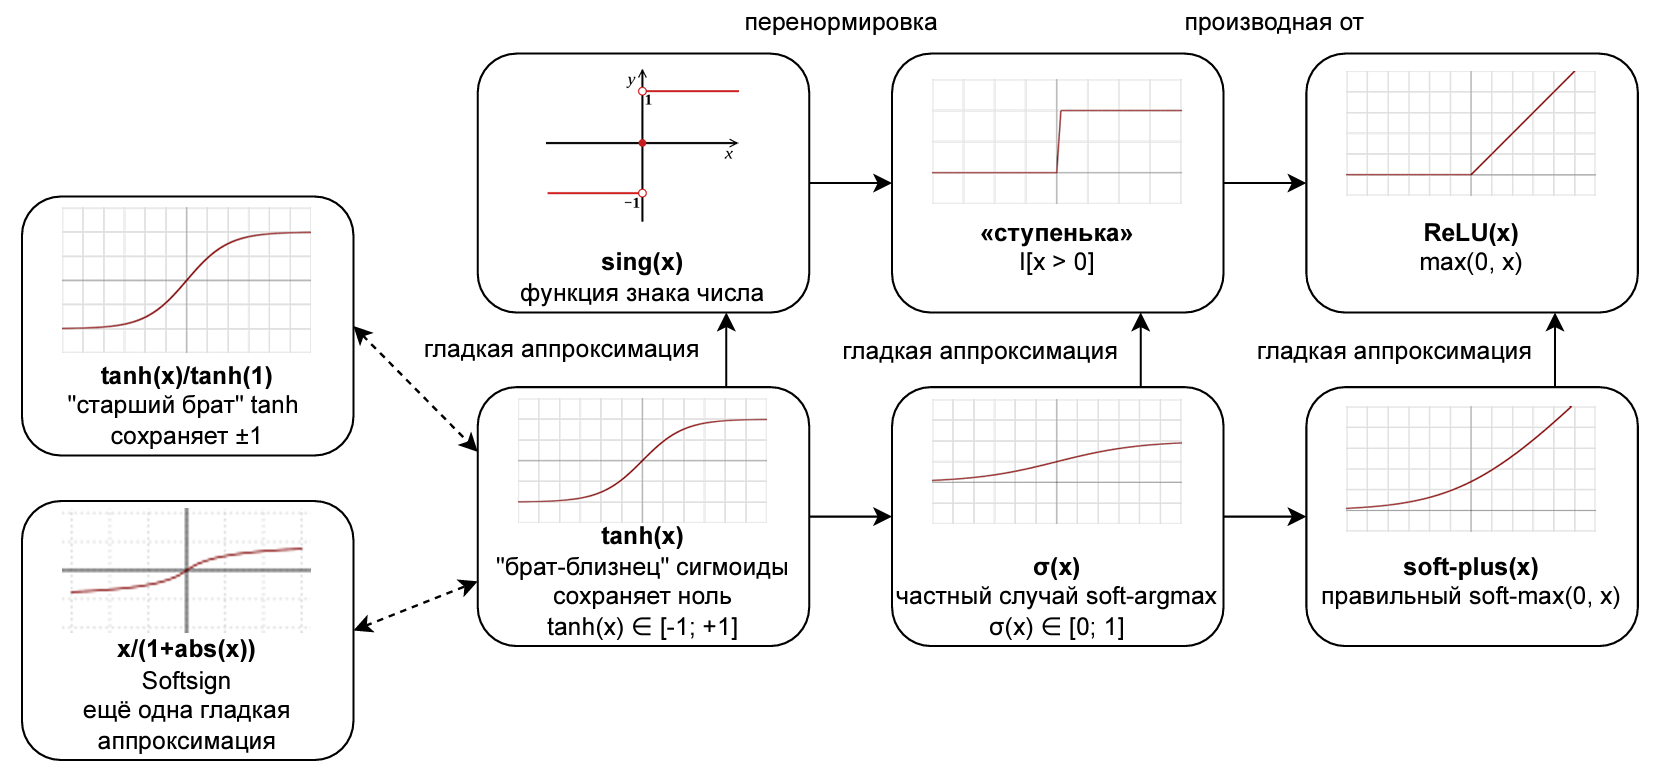
\includegraphics[scale=0.35]{images/connection-of-activation-functions.png}
    \caption{Связь функций активации}
\end{figure}

\section{Декомпозиция моделей}

Еще одно преимущество моделей глубокого обучения в возможности декомпозиции моделей. Например, возможно выполнение переноса знаний: когда у нас уже есть обученная функция и специфическая задача с подходящим входом, мы можем переиспользовать часть уже обученной функции, причем не только её архитектуру, но и её параметры.\newline
Вначале обучения пересчёт производной через ещё не обученные (новые) преобразования будет портить параметры уже обученных (старых) преобразований при обновлении. Поэтому параметры уже обученных преобразований замораживаются (не обновляются). После обучения новых преобразований можно разморозить параметры и дообучить старые преобразования.\newline
Можно выполнять прореживание ResNet архитектуры:
\begin{itemize}
    \item Каждое преобразование имеет "обходной путь".
    \item Бесполезные преобразования будут возвращать близкие к нулю значения.
    \item Следовательно, можно удалить преобразования которые возвращают меньшие значения.
    \item Значения можно оценивать на отдельном (валидационном наборе данных).
    \item После удаления преобразований архитектуру требуется дообучить.
\end{itemize}

Послойные преобразования тоже можно прореживать (выкидывать ребра из графа):
\begin{itemize}
    \item Полносвязное преобразование можно представить двудольным графом.
    \item В этом графе можно удалять (прореживать) рёбра, которые соответствуют наиболее бесполезным параметрам.
    \item Полезность рёбер можно определять по формуле
    \[
        L_i=\dfrac{a_i^2}{[H^{-1}]_{i,i}},
    \]
    где $a_i$ -- значение $i$-го параметра, а $H$ -- гессиан (матрица вторых производных).
    \item Если вторая производная вычисляется долго, то вместо нее можно использовать просто $|a_i|$.
\end{itemize}

\begin{remark}
    После прореживания полносвязных преобразований, также лучше запускать дообучение.
\end{remark}

\section{Дропаут и Батчевая нормализация}

\begin{definition}
    \textbf{Дропаут} (\textit{dropout}) --- преобразование, при котором на итерации обучения обнуляются выходы нейронов с некоторой вероятностью (часто $0.5$).
\end{definition}

\textbf{Преимущества}
\begin{enumerate}
    \item Обнуленные нейроны не участвуют в обучении, не внося вклад в ошибку.
    \item Для каждого выхода фактически строится новая сеть, но у всех этих сетей общие параметры.
    \item Уменьшается соадаптация нейронов, потому что они не могут рассчитывать на соседей.
    \item Обучается более робастное (выбросоустойчивое) представление.
    \item Без дропаута сети значительно переобучаются.
    \item Дропаут приблизительно вдвое увеличивает число операций до сходимости.
\end{enumerate}

\begin{remark}
    Дропаут не идентичен прореживанию, так как на каждой итерации выключаются разные (случайные) нейроны, а в конце обучения они все остаются включенными (никакие ребра не вырезаются).
\end{remark}

\begin{remark}
    Так как на каждой итерации сеть рассчитывает, что нейронов, например, на 30\% меньше, в параметры могут быть на 30\% больше. Когда все нейроны сети включены, может потребоваться сделать поправку.
\end{remark}

\begin{remark}
    Когда меняются параметры слоя, также меняются распределения его выхода.
\end{remark}

\begin{definition}
    \textbf{Батчевая (пакетная) нормализация} --- преобразование, которое старается поддерживать константу ковариации для каждого выходного слоя:
    \[
        \widehat{x}_d=\dfrac{x_d-\E[x_d]}{\sqrt{\D[x_d] + \epsilon}}
    \]
    Пакетный слой пакетной нормализации:
    \[
        \widehat{y}_d=\gamma_d\widehat{x}_d+\beta_d.
    \]
\end{definition}

\begin{remark}
    Такая нормализация называется батчевой, так как математическое ожидание и дисперсия оцениваются по \textit{пакету} данных.
\end{remark}

\begin{remark}
    При применении пакетной нормализации дропаут становится бесполезным.
\end{remark}

\section{Инициализация параметров}

\begin{remark}
    Параметры сдвига можно инициализировать нулями, однако матрицы преобразований нельзя инициализировать нулями или любыми другими одинаковыми значениями, так что принято использовать случайные значения для их инициализации.
\end{remark}

Предположим, что у нас есть функция активации $f$, линейная вблизи $0$ (например, $\tanh$):
\[
    f(x)=x
\]

Рассмотрим нейрон $y$ ($n$ -- число нейронов на предыдущем слое):
\[
    y=\sum_{i=1}^nw_ix_i
\]

Для каждого слоя мы хотим, чтобы дисперсия оставалась одинаковой. Это поможет нам не допустить "взрыва" и затухания градиента. Вычислим дисперсию $y$, считая, что входы и параметры независимы и получены из симметричных равномерных или нормальных распределений:
\[
    \D y=\D\left(\sum_{i=1}^nw_ix_i\right)=\sum_{i=1}^n\D(w_ix_i)=\sum_{i=1}^n\E(w_i^2x_i^2)-\E^2(w_ix_i)=\sum_{i=1}^n\E(w_i^2x_i^2)=
\]
\[
    =\sum_{i=1}^n\E w_i^2\E x_i^2=\sum_{i=1}^n(\E w_i^2-\E^2w_i)(\E x_i^2-\E^2x_i)=\sum_{i=1}^n\D w_i\D x_i=n\cdot\D w_i\cdot\D x_i
\]
Чтобы дисперсия выхода $\D y$ была равна дисперсии входа $\D x$, требуется выполнение следующего условия: $\D w_i=\dfrac{1}{n}$. В целом аналогичный подход, который выполняет некоторое сглаживание между слоями, предлагает брать $\D w_i=\dfrac{1}{\bar{n}}$. Где $\bar{n}$ -- это среднее арифметическое между числом входных нейронов и выходных.

\begin{definition}
    \textbf{Метод инициализации Завьера} (\textit{Xavier}) --- метод, который стремиться упростить прохождение сигнала через слой во время вычисления функции и градиента для линейной вблизи нуля функции активации. При вычислении весов этот метод опирается на вероятностное распределение (равномерное или нормальное) с дисперсией, равной
    \[
        \dfrac{2}{n_{in} + n_{out}},
    \]
    где $n_{in}$ и $n_{out}$ --- это кол-во нейронов на предыдущем и последующем слоях соответственно.
\end{definition}

Для функции активации ReLU, которая не является линейной в области нуля подходит другой метод инициализации.

\begin{definition}
    \textbf{Метод инициализации Ге} (\textit{He}) --- вариация метода Завьера, больше подходящая для функции ReLU, компенсирующая тот факт, что эта функция равна нулю на половине области определения. Дисперсия распределения, из которого необходимо получать начальные значения параметров, полагается равной
    \[
        \dfrac{2}{n_{in}}\quad\text{или}\quad\dfrac{2}{n_{out}}.
    \]
\end{definition}

\begin{remark}
    На практике для функции активации ReLU метод Ге показывает себя значительно лучше, чем метод Завьера.
\end{remark}